 
%% bare_conf.tex
%% V1.4b
%% 2015/08/26
%% by Michael Shell
%% See:
%% http://www.michaelshell.org/
%% for current contact information.
%%
%% This is a skeleton file demonstrating the use of IEEEtran.cls
%% (requires IEEEtran.cls version 1.8b or later) with an IEEE
%% conference paper.
%%
%% Support sites:
%% http://www.michaelshell.org/tex/ieeetran/
%% http://www.ctan.org/pkg/ieeetran
%% and
%% http://www.ieee.org/

%%*************************************************************************
%% Legal Notice:
%% This code is offered as-is without any warranty either expressed or
%% implied; without even the implied warranty of MERCHANTABILITY or
%% FITNESS FOR A PARTICULAR PURPOSE! 
%% User assumes all risk.
%% In no event shall the IEEE or any contributor to this code be liable for
%% any damages or losses, including, but not limited to, incidental,
%% consequential, or any other damages, resulting from the use or misuse
%% of any information contained here.
%%
%% All comments are the opinions of their respective authors and are not
%% necessarily endorsed by the IEEE.
%%
%% This work is distributed under the LaTeX Project Public License (LPPL)
%% ( http://www.latex-project.org/ ) version 1.3, and may be freely used,
%% distributed and modified. A copy of the LPPL, version 1.3, is included
%% in the base LaTeX documentation of all distributions of LaTeX released
%% 2003/12/01 or later.
%% Retain all contribution notices and credits.
%% ** Modified files should be clearly indicated as such, including  **
%% ** renaming them and changing author support contact information. **
%%*************************************************************************


% *** Authors should verify (and, if needed, correct) their LaTeX system  ***
% *** with the testflow diagnostic prior to trusting their LaTeX platform ***
% *** with production work. The IEEE's font choices and paper sizes can   ***
% *** trigger bugs that do not appear when using other class files.       ***                          ***
% The testflow support page is at:
% http://www.michaelshell.org/tex/testflow/



\documentclass[draftcls, onecolumn, peerreview]{IEEEtran}
% Some Computer Society conferences also require the compsoc mode option,
% but others use the standard conference format.
%
% If IEEEtran.cls has not been installed into the LaTeX system files,
% manually specify the path to it like:
% \documentclass[conference]{../sty/IEEEtran}





% Some very useful LaTeX packages include:
% (uncomment the ones you want to load)


% *** MISC UTILITY PACKAGES ***
%
%\usepackage{ifpdf}
% Heiko Oberdiek's ifpdf.sty is very useful if you need conditional
% compilation based on whether the output is pdf or dvi.
% usage:
% \ifpdf
%   % pdf code
% \else
%   % dvi code
% \fi
% The latest version of ifpdf.sty can be obtained from:
% http://www.ctan.org/pkg/ifpdf
% Also, note that IEEEtran.cls V1.7 and later provides a builtin
% \ifCLASSINFOpdf conditional that works the same way.
% When switching from latex to pdflatex and vice-versa, the compiler may
% have to be run twice to clear warning/error messages.






% *** CITATION PACKAGES ***
%
\usepackage{cite}
% cite.sty was written by Donald Arseneau
% V1.6 and later of IEEEtran pre-defines the format of the cite.sty package
% \cite{} output to follow that of the IEEE. Loading the cite package will
% result in citation numbers being automatically sorted and properly
% "compressed/ranged". e.g., [1], [9], [2], [7], [5], [6] without using
% cite.sty will become [1], [2], [5]--[7], [9] using cite.sty. cite.sty's
% \cite will automatically add leading space, if needed. Use cite.sty's
% noadjust option (cite.sty V3.8 and later) if you want to turn this off
% such as if a citation ever needs to be enclosed in parenthesis.
% cite.sty is already installed on most LaTeX systems. Be sure and use
% version 5.0 (2009-03-20) and later if using hyperref.sty.
% The latest version can be obtained at:
% http://www.ctan.org/pkg/cite
% The documentation is contained in the cite.sty file itself.






% *** GRAPHICS RELATED PACKAGES ***
%
\ifCLASSINFOpdf
  \usepackage[pdftex]{graphicx}
  % declare the path(s) where your graphic files are
  % \graphicspath{{../pdf/}{../jpeg/}}
  % and their extensions so you won't have to specify these with
  % every instance of \includegraphics
  \DeclareGraphicsExtensions{.pdf,.jpeg,.png}
\else
  % or other class option (dvipsone, dvipdf, if not using dvips). graphicx
  % will default to the driver specified in the system graphics.cfg if no
  % driver is specified.
  \usepackage[dvips]{graphicx}
  % declare the path(s) where your graphic files are
  % \graphicspath{{../eps/}}
  % and their extensions so you won't have to specify these with
  % every instance of \includegraphics
  % \DeclareGraphicsExtensions{.eps}
\fi
% graphicx was written by David Carlisle and Sebastian Rahtz. It is
% required if you want graphics, photos, etc. graphicx.sty is already
% installed on most LaTeX systems. The latest version and documentation
% can be obtained at: 
% http://www.ctan.org/pkg/graphicx
% Another good source of documentation is "Using Imported Graphics in
% LaTeX2e" by Keith Reckdahl which can be found at:
% http://www.ctan.org/pkg/epslatex
%
% latex, and pdflatex in dvi mode, support graphics in encapsulated
% postscript (.eps) format. pdflatex in pdf mode supports graphics
% in .pdf, .jpeg, .png and .mps (metapost) formats. Users should ensure
% that all non-photo figures use a vector format (.eps, .pdf, .mps) and
% not a bitmapped formats (.jpeg, .png). The IEEE frowns on bitmapped formats
% which can result in "jaggedy"/blurry rendering of lines and letters as
% well as large increases in file sizes.
%
% You can find documentation about the pdfTeX application at:
% http://www.tug.org/applications/pdftex





% *** MATH PACKAGES ***
%
\usepackage{amsmath}
% A popular package from the American Mathematical Society that provides
% many useful and powerful commands for dealing with mathematics.
%
% Note that the amsmath package sets \interdisplaylinepenalty to 10000
% thus preventing page breaks from occurring within multiline equations. Use:
%\interdisplaylinepenalty=2500
% after loading amsmath to restore such page breaks as IEEEtran.cls normally
% does. amsmath.sty is already installed on most LaTeX systems. The latest
% version and documentation can be obtained at:
% http://www.ctan.org/pkg/amsmath





% *** SPECIALIZED LIST PACKAGES ***
%
%\usepackage{algorithmic}
% algorithmic.sty was written by Peter Williams and Rogerio Brito.
% This package provides an algorithmic environment fo describing algorithms.
% You can use the algorithmic environment in-text or within a figure
% environment to provide for a floating algorithm. Do NOT use the algorithm
% floating environment provided by algorithm.sty (by the same authors) or
% algorithm2e.sty (by Christophe Fiorio) as the IEEE does not use dedicated
% algorithm float types and packages that provide these will not provide
% correct IEEE style captions. The latest version and documentation of
% algorithmic.sty can be obtained at:
% http://www.ctan.org/pkg/algorithms
% Also of interest may be the (relatively newer and more customizable)
% algorithmicx.sty package by Szasz Janos:
% http://www.ctan.org/pkg/algorithmicx




% *** ALIGNMENT PACKAGES ***
%
\usepackage{array}
% Frank Mittelbach's and David Carlisle's array.sty patches and improves
% the standard LaTeX2e array and tabular environments to provide better
% appearance and additional user controls. As the default LaTeX2e table
% generation code is lacking to the point of almost being broken with
% respect to the quality of the end results, all users are strongly
% advised to use an enhanced (at the very least that provided by array.sty)
% set of table tools. array.sty is already installed on most systems. The
% latest version and documentation can be obtained at:
% http://www.ctan.org/pkg/array


% IEEEtran contains the IEEEeqnarray family of commands that can be used to
% generate multiline equations as well as matrices, tables, etc., of high
% quality.




% *** SUBFIGURE PACKAGES ***
%\ifCLASSOPTIONcompsoc
%  \usepackage[caption=false,font=normalsize,labelfont=sf,textfont=sf]{subfig}
%\else
%  \usepackage[caption=false,font=footnotesize]{subfig}
%\fi
% subfig.sty, written by Steven Douglas Cochran, is the modern replacement
% for subfigure.sty, the latter of which is no longer maintained and is
% incompatible with some LaTeX packages including fixltx2e. However,
% subfig.sty requires and automatically loads Axel Sommerfeldt's caption.sty
% which will override IEEEtran.cls' handling of captions and this will result
% in non-IEEE style figure/table captions. To prevent this problem, be sure
% and invoke subfig.sty's "caption=false" package option (available since
% subfig.sty version 1.3, 2005/06/28) as this is will preserve IEEEtran.cls
% handling of captions.
% Note that the Computer Society format requires a larger sans serif font
% than the serif footnote size font used in traditional IEEE formatting
% and thus the need to invoke different subfig.sty package options depending
% on whether compsoc mode has been enabled.
%
% The latest version and documentation of subfig.sty can be obtained at:
% http://www.ctan.org/pkg/subfig




% *** FLOAT PACKAGES ***
%
%\usepackage{fixltx2e}
% fixltx2e, the successor to the earlier fix2col.sty, was written by
% Frank Mittelbach and David Carlisle. This package corrects a few problems
% in the LaTeX2e kernel, the most notable of which is that in current
% LaTeX2e releases, the ordering of single and double column floats is not
% guaranteed to be preserved. Thus, an unpatched LaTeX2e can allow a
% single column figure to be placed prior to an earlier double column
% figure.
% Be aware that LaTeX2e kernels dated 2015 and later have fixltx2e.sty's
% corrections already built into the system in which case a warning will
% be issued if an attempt is made to load fixltx2e.sty as it is no longer
% needed.
% The latest version and documentation can be found at:
% http://www.ctan.org/pkg/fixltx2e


% *** PDF, URL AND HYPERLINK PACKAGES ***
%
\usepackage{url}
% url.sty was written by Donald Arseneau. It provides better support for
% handling and breaking URLs. url.sty is already installed on most LaTeX
% systems. The latest version and documentation can be obtained at:
% http://www.ctan.org/pkg/url
% Basically, \url{my_url_here}.

%============================================================================
%============================================================================

% correct bad hyphenation here
\hyphenation{op-tical net-works semi-conduc-tor}

%%%%%%%%%%%%%%%%%%%%%%%%%%%%%%%%%%%%%%%%%%%%%%%%%%%%%%%%%%%%%%%%%%%%%%%%%%%%%%
%%%%%%%%%%%%%%%%%%%%%%%%%%%%%%%%%%%%%%%%%%%%%%%%%%%%%%%%%%%%%%%%%%%%%%%%%%%%%%

\usepackage{booktabs}

\usepackage{hyperref}

%*** Other packages included by Julio Eciso
\usepackage{ bbold }         % fancy symbol for the vector of 1's
\usepackage{amsfonts}        % symbols for real numbers, etc

\usepackage{lineno}

%*** Custom commands by Julio Enciso
\newcommand{\R}{\mathbb{R}}

%\DeclareMathOperator*{\argmax}{arg\,max}
\DeclareMathOperator*{\argmin}{arg\,min}

%%%%%%%%%%%%%%%%%%%%%%%%%%%%%%%%%%%%%%%%%%%%%%%%%%%%%%%%%%%%%%%%%%%%%%%%%%%%%%
%%%%%%%%%%%%%%%%%%%%%%%%%%%%%%%%%%%%%%%%%%%%%%%%%%%%%%%%%%%%%%%%%%%%%%%%%%%%%%

\begin{document}

\linenumbers % Lineno command, turn on line numbering.
%
% paper title
% Titles are generally capitalized except for words such as a, an, and, as,
% at, but, by, for, in, nor, of, on, or, the, to and up, which are usually
% not capitalized unless they are the first or last word of the title.
% Linebreaks \\ can be used within to get better formatting as desired.
% Do not put math or special symbols in the title.
\title{A Robust ECoG Source Localization Method Using Brain Data Analytics Validated by Pig Intracerebral Recordings}


% author names and affiliations
% use a multiple column layout for up to three different
% affiliations
\author{
\IEEEauthorblockN{Julio Cesar Enciso-Alva}
\IEEEauthorblockA{(University of Texas at Arlington)\\
Arlington, Texas, 76019\\
%Email: 
juliocesar.encisoalva@mavs.uta.edu}
\par
\and
\IEEEauthorblockN{Aksharkumar Dobariya}
\IEEEauthorblockA{(UT Southwestern Medical Center)\\
Dallas, Texas, 75390\\
%Email: 
aksharkumar.dobariya@utsouthwestern.edu}
\par
\and
\IEEEauthorblockN{Talon Johnson}
\IEEEauthorblockA{(University of Texas at Arlington)\\
Arlington, Texas, 76019\\
%Email: 
talon.johnson@mavs.uta.edu}
\par
\and
\IEEEauthorblockN{Bruce Mickey}
\IEEEauthorblockA{(UT Southwestern Medical Center)\\
% Dept. Neurological Surgery
Dallas, Texas, 75390\\
%Email: 
}
\par
\and
\IEEEauthorblockN{Juan M. Pascual}
\IEEEauthorblockA{(UT Southwestern Medical Center)\\
Dallas, Texas, 75390\\
%Email: 
juan.pascual@utsouthwestern.edu}
\par
\and
\IEEEauthorblockN{Jiangzhong Su}
\IEEEauthorblockA{(University of Texas at Arlington)\\
Arlington, Texas, 76019\\
%Email: 
su@uta.edu}
}

% make the title area
\maketitle

% As a general rule, do not put math, special symbols or citations
% in the abstract
\begin{abstract}
Brain electric signal source localization has become useful for studying brain activation patterns. 
Electrical activity inside the brain can be modeled as a current density distribution via a collection of equivalent dipoles located on a regular grid,
whose magnitudes and momentum are
determined using recordings of electric potentials at the surface of the head. 
The process is known as Electrical Source Imaging with unconstrained dipoles and constitutes an ill-posed inverse Poisson problem. This problem can be solved efficiently using multiple algorithms,
from which we highlight 
minimum-norm algorithms such as sLORETA (standardized Low-Resolution Electromagnetic Tomography Analysis). 
However, the validity of these methods is often verified through computer-simulated data.  Few studies have validated the source localization methods in human or animal models. \\
Simultaneous recordings of electrocorticography (ECoG) and deep electrodes allow us to compare 
estimations from Electrical Source Imaging against recordings from electrodes inserted on the brain volume.
In this study, we assess the performance of a proposed minimum-norm algorithm for the ECoG reconstruction method, using data from pig brain experiments during different stages of an induced lesion. 
This methodology is demonstrated using data from an animal model, displaying complex events.
Our finding supports 
that estimations from Electrical Source Imaging capture similar activity patterns as the deep electrodes. 
\end{abstract}

% no keywords

\IEEEpeerreviewmaketitle

%============================================================================
%============================================================================

\section{Introduction}
% no \IEEEPARstart

A central task for many fields in neuroscience is to determine the location of activity inside the brain.
%
Electrical activity in particular is known for the high temporal resolution at which it can be recorded, possibly at a sub-millisecond scale.
%
On the other side, electrical recordings of neural activity are also known to have a very poor spatial resolution, thus making it difficult to locate unambiguously the location of such activity 
\cite{baillet_intro}.
 
In order to locate this electrical activity inside the brain, such activity is usually modeled via a collection of electrical dipoles.
%
The characterization of these dipoles may assume unknown locations and magnitudes (parametric), or a finite set of equivalent dipoles with known locations and orientation over a grid covering the anatomical space of interest (non-parametric)
%
\cite{classic_models}. 

Non-parametric estimation is often preferred when the location of the anatomical generators of the activity of interest is either unknown  or extended over a relatively large area.
%
Such estimation can be formulated as an inverse Poisson problem which happens to be ill-posed; it is under-determined and thus, it doesn't have a unique solution
\cite{hallez_review}.

Additional assumptions are often added to alleviate the ill-posed nature of the problem of source estimation.
%
One of those assumptions is that, among all the possible solutions for the problem, the more feasible estimations are those representing lower total energy; this quantity is modeled as a vector norm, and thus the estimations obtained are referred to as minimal-norm solutions.
%
%
There are multiple algorithms that solve efficiently the minimal-norm source estimation problem
\cite{eeg_source_location}.


Although parametric electrical source reconstruction is usually performed using recordings of electroencephalography (EEG) or magnetoencephalography (MEG),  it is possible to use different modalities such as electrocorticography (ECoG) \cite{ecog_other}.

Both EEG and MEG have sensors positioned near or in contact with the subject's scalp, while ECoG requires electrodes placed over the patient's brain surface thus being invasive.
%
ECoG recordings are not subject to the attenuation caused by the multiple layers of tissue that separate the brain from the scalp, including the skull.
%
Deep electrodes inserted on the subject's brain are more invasive than ECoG and have more restrictions on where they can be placed, but have better spatial resolution.

For this study, a peculiar setup is considered which consists of simultaneous recordings from ECoG and deep electrodes inside the brain.
%
This arrangement was applied to a study of ischemic stroke on the pig.
%
We had previously described the recording methodology and determined that pig ECoG was virtually indistinguishable from human ECoG \cite{PMID_36109613}.

By using the methodology of electrical source reconstruction from ECoG data, it is possible to estimate recordings that could be obtained from deep electrodes at arbitrary locations; we refer to these estimations as recordings from virtual deep electrodes.
%
The main goal of this work is to assess the usability of using virtual deep electrodes, computed from ECoG data, in comparison with recordings from real deep electrodes.
%
As the correspondence may be imperfect, the performance metric is based on a task of automatic burst detection.

Multiple authors have explored the concept of virtual sensors, estimated from MEG/EEG data via electrical source reconstruction, in the study of epilepsy in humans \cite{hillebrand2005new,tamilia2021noninvasive,sohrabpour2020noninvasive}. 
%
One additional goal of this work is to propose the usability of this tool in the study of stroke in humans, given that an animal model has been already established.

%============================================================================
%============================================================================

\section{Methods}

\subsection{Data collection in Animal Model}

ECoG data was collected from a domestic pig during a study of acute ischemic stroke in the right middle central artery on animal models \cite{PMID_36109613}.
%
The protocol of that study was approved by the Institutional Animal Care and Use Committee of UT Southwestern Medical Center, in addition to ARRIVE (Animal Research: Reporting of In Vivo Experiments) guidelines.

Following a protocol similar to that of \cite{pig_lesion1}, the subject was kept anesthetized using isoflurane and underwent a craniotomy in order to expose the brain. 
%
Ischemia was induced by cauterization or clamping (using an aneurysm clip) of the right middle central artery; this process will be referred to as the \textit{induced lesion}.

Electrophysiological recordings were obtained at a sampling frequency of 1 kHz during three conditions for 10 minutes each:
%recordings were digitized at 1 kHz for intervals of 10 minutes during three conditions: 
previous to the lesion, immediately after the lesion, and 60 minutes after the lesion.
%
Only the first two conditions are accounted for in the analysis.

The ECoG montage consisted of 
two $4\times 1$ electrode strips
(4.5 mm radius for contact, 0.76 mm thick, 10 mm center-to-center, textured surface)
placed directly on the cortex surface,
%
Each strip was placed parallel to and 10 mm away from the medial line, and 10 mm away from the anterior edge.
%
Two ECoG electrodes were excluded due to disconnection.

The montage of Deep electrodes consisted of two stylets of 
8 macro-depth electrodes each
(1.28 mm stylet thick, 1.57 mm electrode length, 5.0 mm center-to-center),
implanted in the craniocaudal direction with entry points between the second and third ECoG strips. 

For a visual reference of the electrode locations, see figure \ref{fig:elecs}.




\begin{figure}[!t]
\centering
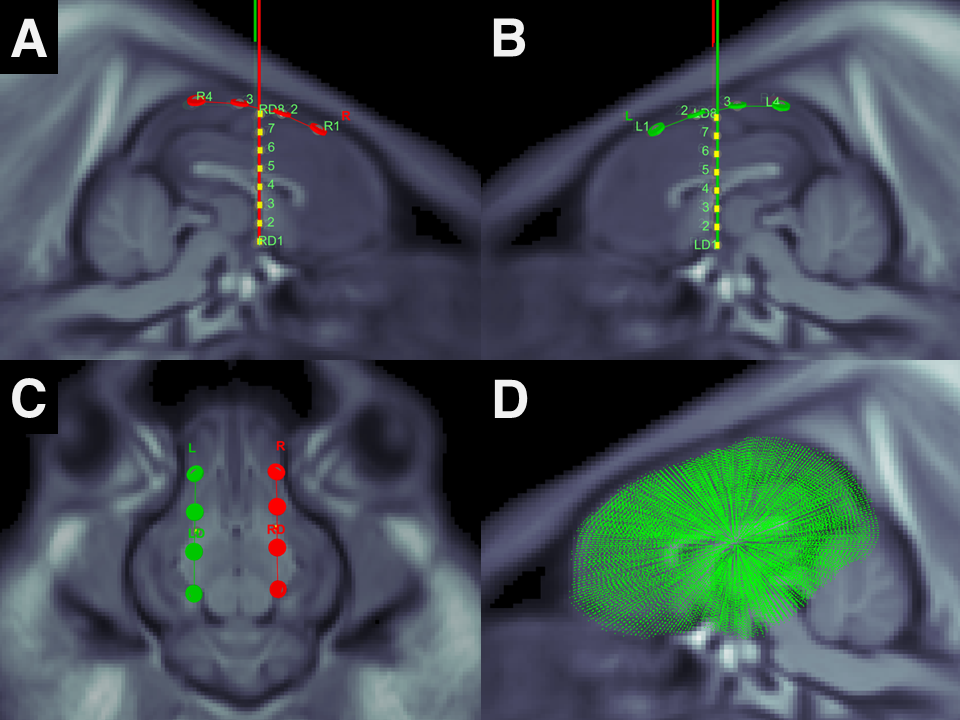
\includegraphics[width=8cm]{./img/electrodes_v2}
\caption{Locations of recording electrodes and distributed dipoles against anatomical MRI.
\textbf{(A-C)} Locations of ECoG electrodes, R1-R4 and L1-L4, and deep electrodes, RD1-RD8 and LD1-LD8. Stereotaxic views from right, left, and top. 
\textbf{(D)} Locations of distributed dipoles; each green dot represents a dipole location. }
\label{fig:elecs}       % Give a unique label
\end{figure}

%============================================================================
%============================================================================

\subsection{Anatomical Data Processing}

In lieu of an anatomical MRI of the subject, a publicly available template was used
\cite{pig_template}.
%
The template was processed via linear warping (rescaling) to match measurements of the subject's brain obtained post-mortem.

Electrode placement was replicated over the template following the experiment guidelines, and 
later they
%
%Electrode locations 
were corrected using fluoroscopy imaging of the subject.

The distributed dipoles were placed using a cubic mesh with 1.0 mm between neighboring points,
resulting in [] dipole locations.
%The positions for the distributed dipoles were decided by generating a layered grid from the cortex surface with $<2$ mm between neighboring locations, resulting in 72,837 dipole locations.
%
Dipoles were assumed to have unknown orientations, thus being each one equivalent to 3 superimposed dipoles with canonical stereotaxic orientations.
%
This grid was created independently of the position of any electrodes 
in order to avoid biases in the reconstruction.
%
%This was done to avoid biases in the comparison of reconstructed data with its ground truth.
%
For a visual reference of the dipole locations, see figure \ref{fig:elecs}.

%============================================================================
%============================================================================

\subsection{Forward Model Solution}

Within the paradigm of non-parametric estimation of electrical sources, the relationship between the dipoles' magnitude and ECoG measurements can be modeled via the matrix equation \eqref{eq:main}. 
%
\begin{equation}
    Y = G\, J + \varepsilon
    \label{eq:main}
\end{equation}

In equation \eqref{eq:main}, $Y$ is a $M\times T$ matrix representing recordings from $M$ sensors at $T$ timestamps, $J$ is a $3N\times T$ matrix representing the magnitudes of $3N$ dipoles --superimposed at $N$ locations, at 3 stereotaxic orientations-- at the same $T$ timestamps, and $\varepsilon$ is a $M\times T$ matrix representing external noise captured by the sensors. 
%
The matrix $M\times 3N$ $G$, also known as leadfield matrix or transfer matrix, represents the generation of the observable electrical potential field from the combination of dipole current density.
%
The task of computing the leadfield matrix is a key component in the forward model.

The theoretical derivation of the leadfield matrix follows from the quasi-static case from the Maxwell equations with the dipoles as only sink/sources and isotropic conductivity. 
%
This formulation is equivalent to a Poisson equation over the geometric domain of the subject head; such domain is often decomposed based on the different tissues --brain, cerebrospinal fluid, skull, etc.--, each one with constant conductivity.
%
Each column of the leadfield matrix is obtained by solving such a problem for each dipole position with unitary magnitude.
%
More detailed and clear descriptions of this process have been published by multiple authors, such as Hallez \cite{hallez_review}.

For the present work, only the brain volume is considered since it is in almost direct contact with the air. 

%============================================================================
%============================================================================

\subsection{Inverse Problem Solution}

From the forward model equation \eqref{eq:main} it is clear that, if the number of dipoles is larger than the number of sensors, then the determination of dipoles' magnitude is an under-determined problem, and thus ill-posed.

A unique solution can be obtained by considering additional constraints, such as looking for the solution with minimal norm.
%
For instance, the sLORETA algorithm considers the penalized inverse problem that can be described as in equation \eqref{eq:sloreta} \cite{sloreta}.
\begin{equation}
    \hat{J} = \argmin_{c,J} \left\Vert Y - G\, J - \mathbb{1} c \right\Vert_F^2 + \alpha \left\Vert J \right\Vert_F^2
    \label{eq:sloreta}
\end{equation}

In equation \eqref{eq:sloreta} $\hat{J}$ is the estimator of $J$,
$\left\Vert J \right\Vert_F^2$ is the Frobenius norm (sum of squares of each entry),
$c$ is a $1\times T$ vector, $\mathbb{1}$ is a $1\times M$ vector of ones, and $\alpha>0$ is a penalization parameter.

By minimizing equation \eqref{eq:sloreta} over $c$, it is found that the optimal each entry must be the average over space of the residual, as in equation \eqref{eq:error} with $e_i$ an $T\times 1$ unitary vector with its $i$-th entry of 1.
\begin{equation}
    c_i = (Y-G\, J) e_i
    \label{eq:error}
\end{equation}

The regularized problem of sLORETA has a solution with a known solution, displayed inequation \eqref{eq:sloreta_sol}.
\begin{equation}
    \hat{J} = {G}^T H \left[ H\, {G} {G}^T H + \alpha H \right]^\dagger Y
    \label{eq:sloreta_sol}
\end{equation}

In equation \eqref{eq:sloreta_sol}, $H$ is a $M\times M$ centering operator defined as 
$H = Id - \mathbb{1} \mathbb{1}^T / \mathbb{1}^T \mathbb{1}$, and $Q^\dagger$ represents the Moore-Penrose pseudo-inverse of the matrix $Q$.

It is relevant to mention that the estimator $\hat{J}$ in equation \eqref{eq:sloreta_sol} is linear, in the sense that it can be written as a linear filter applied to the sensor data as in equation \eqref{eq:kernel}.

\begin{equation}
    \begin{cases}
        \hat{J} &= W\, Y \\
        W &=
        {G}^T H \left[ H\, {G} {G}^T H + \alpha H \right]^\dagger
    \end{cases}
    \label{eq:kernel}
\end{equation}

For this work, the inverse solution is computed using the sLORETA implementation from the Brainstorm toolbox. 
%
This implementation does not directly compute $\hat{J}$, but instead the inversion kernel $W$ from equation \eqref{eq:kernel}.

The leadfield matrix $G$ is obtained from the forward head model described in the previous section, and the parameter $\alpha$ is set to the square root median eigenvalue of $G\, G^T$.

%============================================================================
%============================================================================

\subsection{Virtual Deep Electrodes from ECoG data}
\label{sec:method_est}

Once the inverse solution was computed, the resulting data was used to simulate recordings that would be obtained by theoretical deep electrodes located at arbitrary locations inside the brain.
%
For each of these virtual deep electrodes, a volume scout is created by considering a sphere with its center at the electrode location and a radius of 3 mm.
%
The magnitudes of dipoles inside each scout are averaged over space in each canonical direction, thus obtaining a time series representing the recordings from that virtual electrode. 
%
See figure \ref{fig:raw} for a visual representation of this process, and figure \ref{fig:control} for an example of recordings from virtual channels.

For this work in particular, for each deep electrode, a virtual electrode is established at the same location.
%
On a conceptual level, virtual electrodes are computed independently of deep electrodes.

\begin{figure}[!t]
\centering
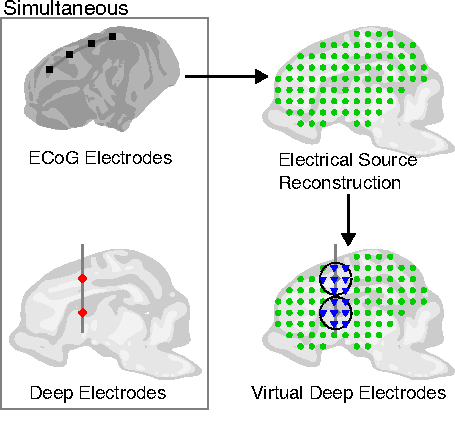
\includegraphics[width=7cm]{./img/diagram_v2}
\caption{Recordings from deep electrodes are simulated using data from electrical source reconstruction, which is based on ECoG data. This is done by averaging the estimated magnitude of all the dipoles near ($<4$ mm) the location of each deep electrode.
}
\label{fig:raw}
\end{figure}

\begin{figure}[!t]
    \centering
    \begin{tabular}{rr}
    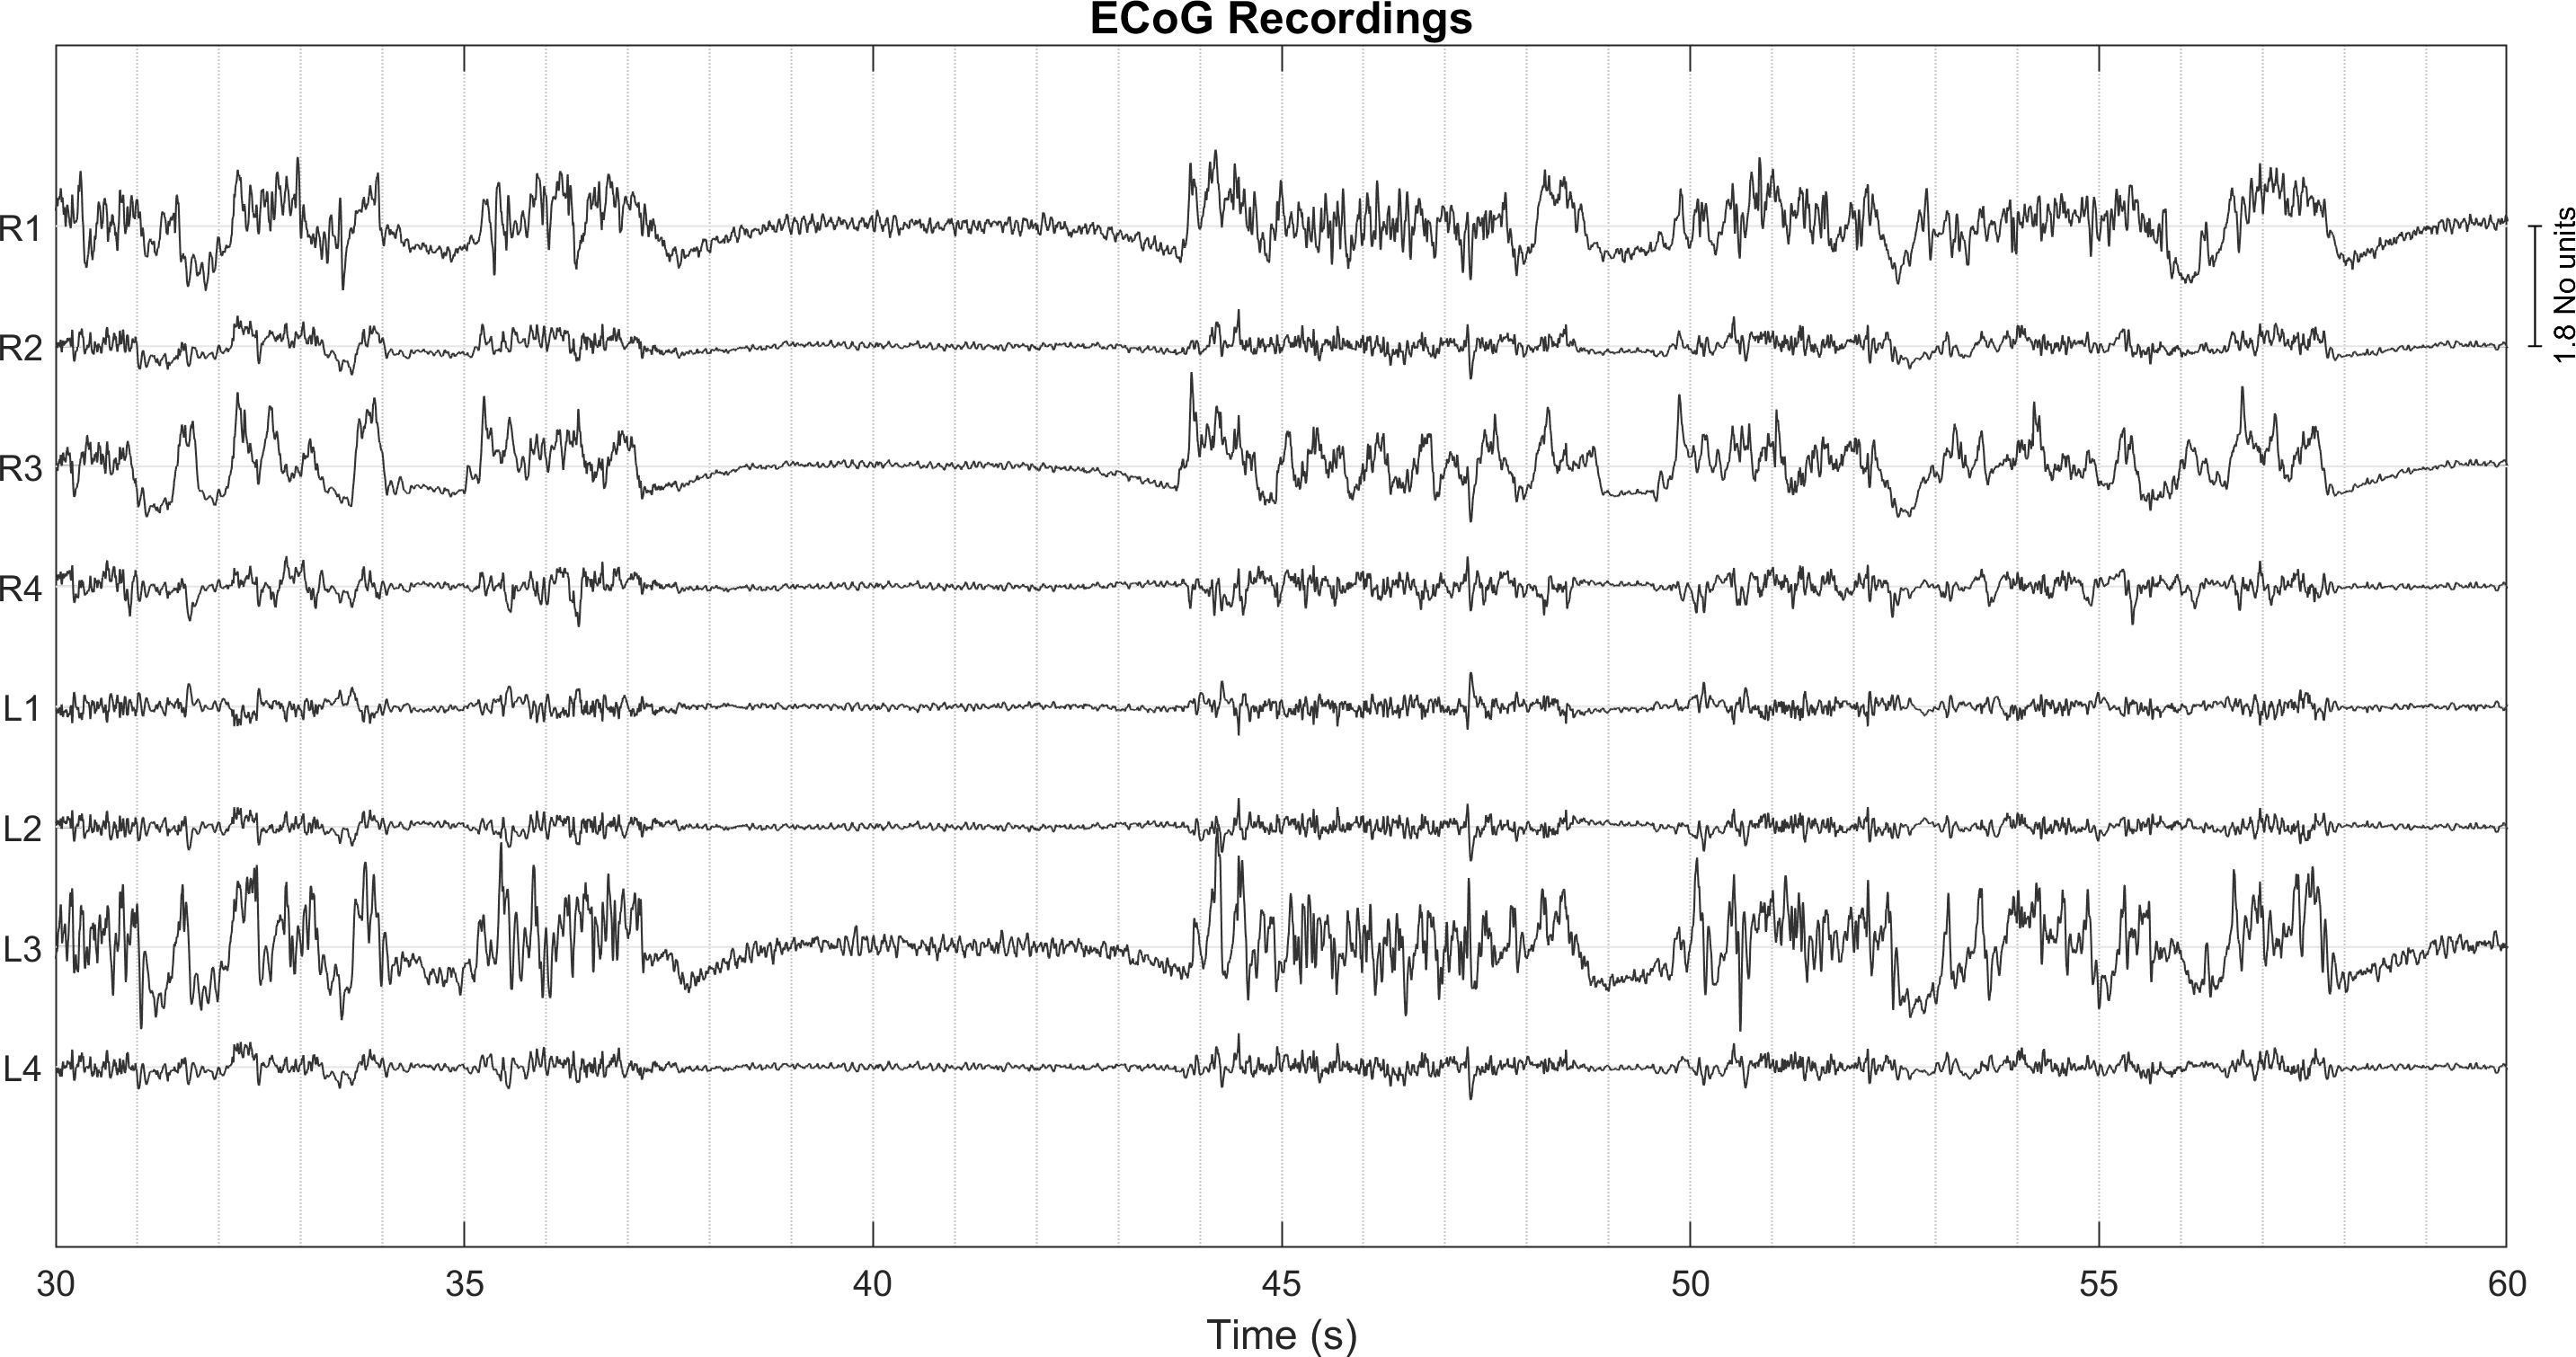
\includegraphics[width=7.75cm]{./img/ctrl_ecog} \\
    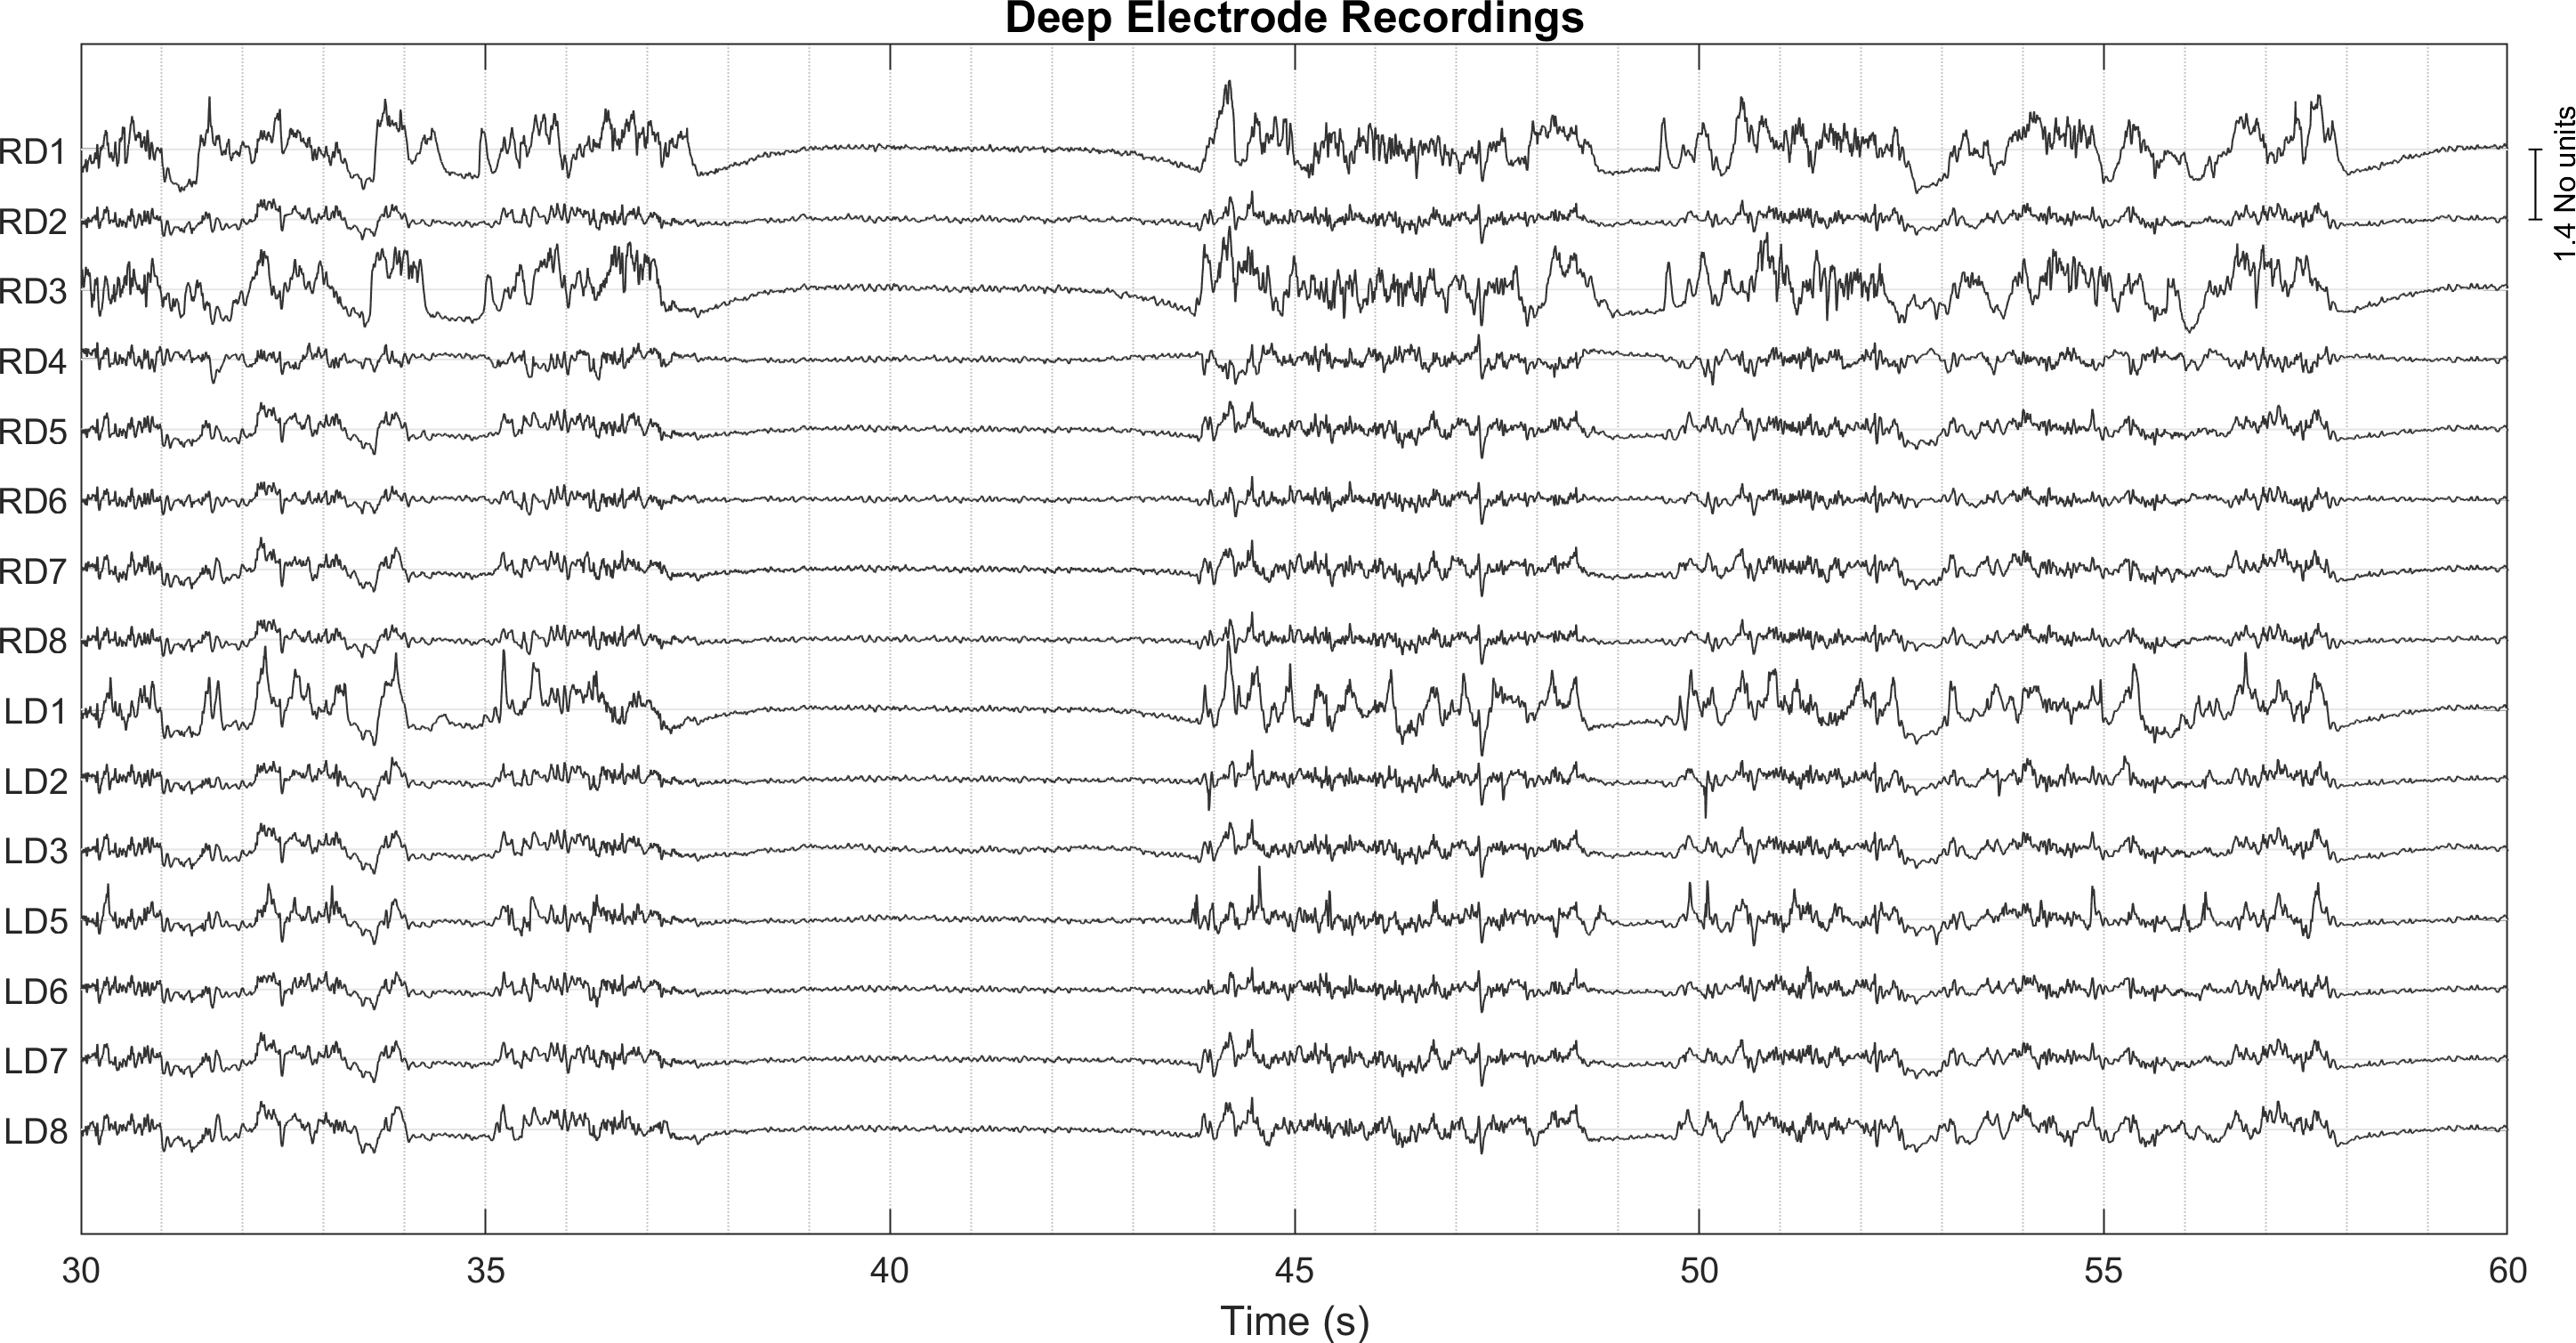
\includegraphics[width=7.8cm ]{./img/ctrl_seeg} \\
    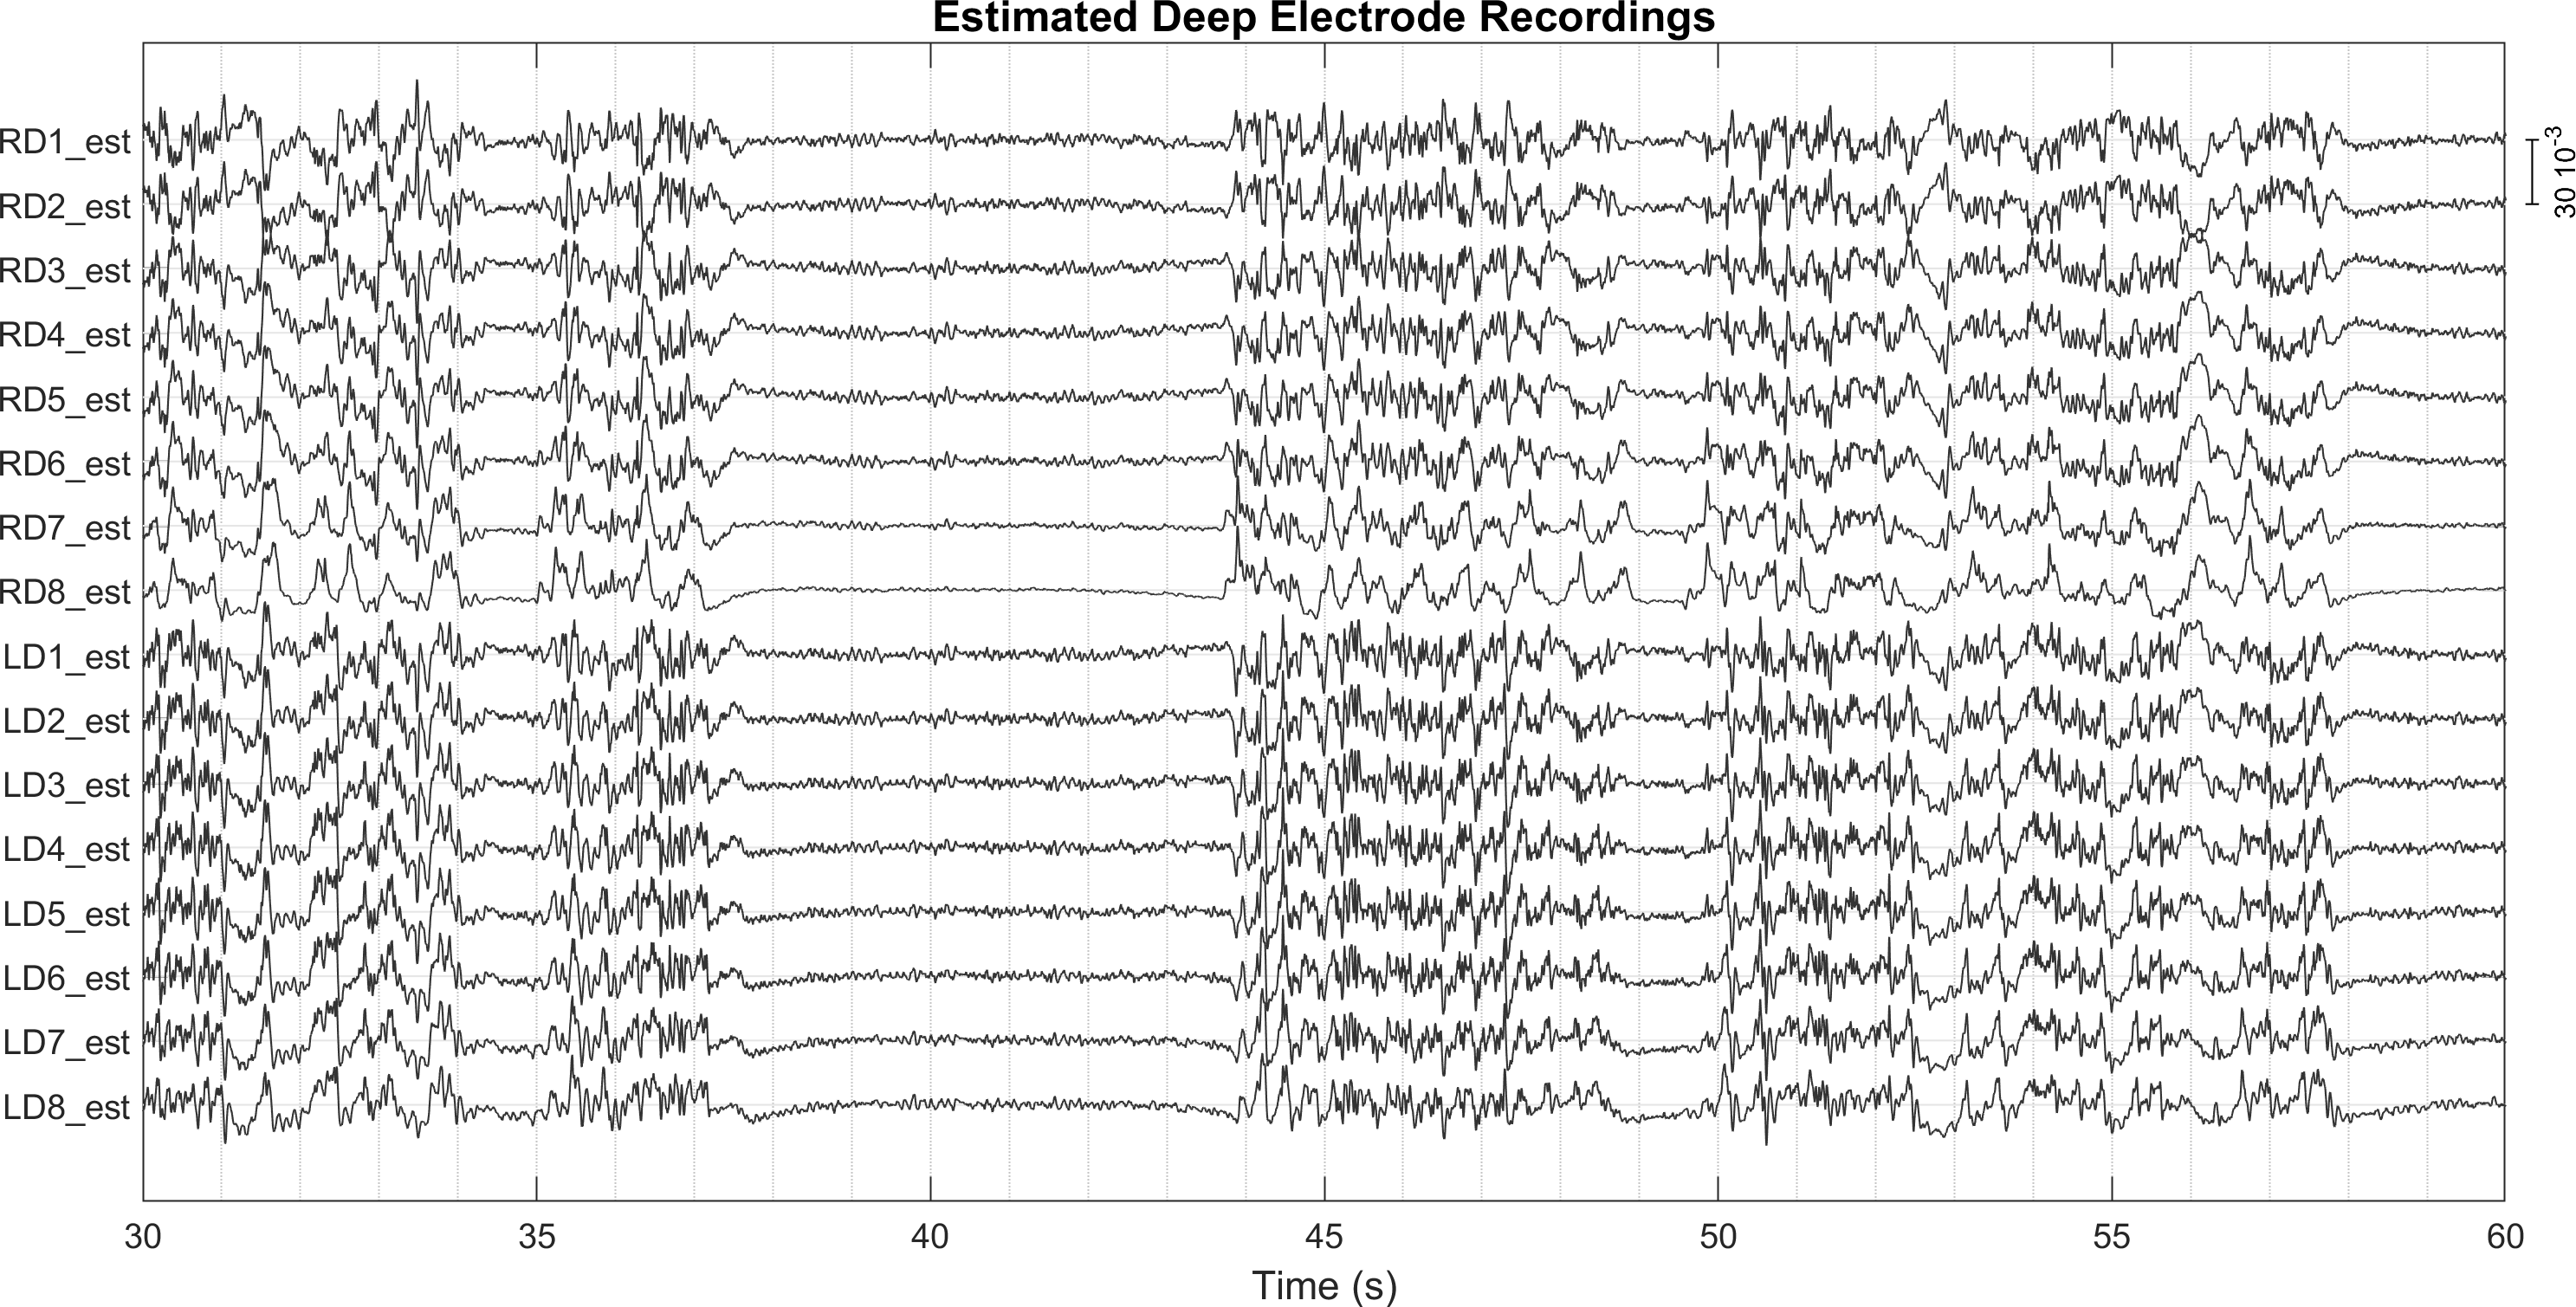
\includegraphics[width=8cm   ]{./img/ctrl_estim}
    \end{tabular}
\caption{Visual comparison of (up) recordings from ECoG electrodes at the cortex surface, (middle) recordings from deep electrodes inserted in the brain volume, and (down) `recordings' from virtual deep electrodes as described in Section \ref{sec:method_est}. This time window of 30 seconds corresponds to a baseline, before the induced lesion.}
    \label{fig:control}
\end{figure}

%============================================================================
%============================================================================

\subsection{Implementation}

The algorithms described in this section for Electrical Source Reconstruction were carried out using the open-source toolbox

Brainstorm \cite{brainstorm} running on MATLAB 2021b \cite{matlab}.

Segmentation of anatomical MRI and extraction of the brain cortex was performed using the CAT toolbox \cite{cat12}. 
%
Multiple artifacts were found while processing the subject's MRI, so we utilized a second version of the same anatomical MRI that had undergone a skull-stripping procedure; such MRI was made publicly available from the same authors \cite{pig_template}.
%
This was done in order to the tissues surrounding the brain, as they differ too much from human anatomy.

Both the pre-processing of the anatomical MRI and the placing of electrodes were performed manually.

The Poisson equations of the forward problem were solved numerically using a Boundary Element model constructed using the cortex surface extracted from the template MRI, as well as the positions of ECoG and deep electrodes.
%
This process was performed using the OpenMEEG toolbox \cite{openmeeg}.

The creation of virtual electrodes was implemented on Matlab with a data format compatible with the Brainstorm toolbox.
%
The code is available on the GitHub page of the author,
\url{https://github.com/EncisoAlva/VirtualDeepElectrodes}.

%============================================================================
%============================================================================

\section{Results}

\subsection{Statistical Correlation and Consistency}
In order to do that, first the statistical reliability of these Virtual Deep Electrodes is explored.

The statistical reliability of Virtual Deep Electrodes is examined by computing the power spectrum over different time windows, using independently the recordings from Deep Electrodes and Virtual Deep Electrodes, and then computing the Spearman Rank Correlation Coefficient (CC) and the Intraclass Correlation Coefficient (ICC).

Recordings are divided into epochs of 30 seconds, and the relative power spectrum (via Fast Fourier Transform) is computed for each channel in the following frequency bands:
{$\delta$=2--4 Hz}, {$\theta$=5--7 Hz}, {{$\alpha$=8--12 Hz}}, {$\beta$=15--30 Hz}, {$\gamma_1$=30--60 Hz}, {$\gamma_2$=60--90 Hz}.

The results, which are shown in table \ref{tab:icc_relative}, display that the Virtual Deep Electrodes become progressively less precise following the induced lesion on the subject. 
%
The observed deterioration is stronger in higher frequencies.

\begin{table*}[!t]
\renewcommand{\arraystretch}{1.3}
\caption{Correlation and Consistency for Relative Power computed from Virtual and Real Deep Electrodes. Marks represent p-value range, o: $p<0.1$, *:$p<0.05$, **:$p<0.01$, ***:$p<0.005$.}
\centering
\begin{tabular}{@{}lrllllrllllrlll@{}}
\toprule
       & \multicolumn{4}{l}{Pre-lesion} &  & \multicolumn{4}{l}{Post-lesion (0 s)}  &  & \multicolumn{4}{l}{Post-lesion (60 s)} \\
       \cmidrule(l){2-5} 
       \cmidrule(l){7-10}
       \cmidrule(l){12-15} 
       & Corr   &      & ICC   &     &  & Corr  &     & ICC   &     &  & Corr     &   & ICC     &   \\ 
       \midrule 
$\delta$
& 0.380  & o    & 0.412 & *   &  & 0.653 & **  & 0.815 & *** &  & 0.006    &   & 0.022   &    \\
$\theta$  
& 0.660  & ***  & 0.780 & *** &  & 0.672 & **  & 0.677 & *** &  & -0.253   &   & -0.126  &    \\
$\alpha$  
& 0.638  & ***  & 0.876 & *** &  & 0.843 & *** & 0.788 & *** &  & 0.183    &   & 0.317   & o  \\
$\beta$   
& 0.829  & ***  & 0.664 & *** &  & 0.715 & **  & 0.345 & o   &  & 0.000    &   & 0.033   &    \\
$\gamma_1$ 
& 0.868  & ***  & 0.419 & *   &  & 0.796 & *** & 0.014 &     &  & 0.185    &   & 0.086   &    \\
$\gamma_2$ 
& 0.711  & ***  & 0.475 & *   &  & 0.763 & *** & 0.017 &     &  & 0.332    &   & 0.299   & o \\
\bottomrule
\end{tabular}
\label{tab:icc_relative}
\end{table*}

Statistical analyses were performed using R version  4.3.2 \cite{R_software}. The Intraclass Correlation Coefficient was computed using the irr package \cite{irr}. 

%============================================================================
%============================================================================

\subsection{Automatic Detection of Bursts}

Once the statistical reliability of Virtual Deep Electrodes is established, the relative power spectrum is later computed at a higher resolution in time via Morlet wavelets (time resolution=3 s, frequency resolution=1 Hz), grouping the same frequency bands; timestamps in the time-frequency domain are set to be the same as in the time domain (1 KHz).

In the most typical case, automatic detection of bursts of high-amplitude activity is performed by setting a threshold, relative to baseline activity, and classifying a segment as part of a burst if the total power exceeds such threshold.
%
The classification is performed over the power spectrum of the frequency bands since it is equivalent to prior filtering of the signal.

We found it relevant to observe the effect of the threshold against the classification accuracy since it addresses a known bias of minimal-norm algorithms based on L2 norm.
%
By design, minimal-norm algorithms are designed to minimize the L2 norm of the reconstruction error. 
%
As a result, solutions tend to have a high number of non-zero entries with relatively low amplitude.
%
The effect of this type of noise can be diminished by tuning the cut-off threshold.

The automatic detection is performed over multiple selections of thresholds for both the Virtual Deep Electrodes and the real Deep Electrodes, and the agreements between those classifications are measured using the following metrics:
\begin{align}
\begin{split}
    \text{Agreement} &= \frac{\text{TP}+\text{TN}}{\text{TP}+\text{FP}+\text{TN}+\text{FN}} \\
    \text{Intersect-over-Union} &= \frac{\text{TP}}{\text{TP}+\text{FP}+\text{FN}} \\
    \text{Precision} &= \frac{\text{TP}}{\text{TP}+\text{FP}} \\
    \text{Recall} &= \frac{\text{TP}}{\text{TP}+\text{FN}}
\end{split}
\end{align}
where TP=True Positive, TN=True Negative, FP=False Positive, TN=True Negative, FN=False Negative. 
%
A True Positive is understood as a segment that was classified as `burst' by using both the Virtual Deep Electrodes and real Deep Electrodes, a False Positive refers to a segment classified as `burst' using Virtual Deep Electrodes and as `no-burst' using real Deep Electrodes; True Negatives and False Negatives are defined analogously.

The evaluation metrics for different thresholds are displayed in figure \ref{fig:band}.
%
The classifications done using a signal filtered to $\gamma_1$ or $\gamma_2$ are imprecise independently of the threshold used. 
%
The frequency bands that offer the best performance on the selected metrics are $\delta$ and $\beta$, and the thresholds that better deal with the reconstruction noise are below 150\% of the baseline power.

\begin{figure*}[!t]
\centering
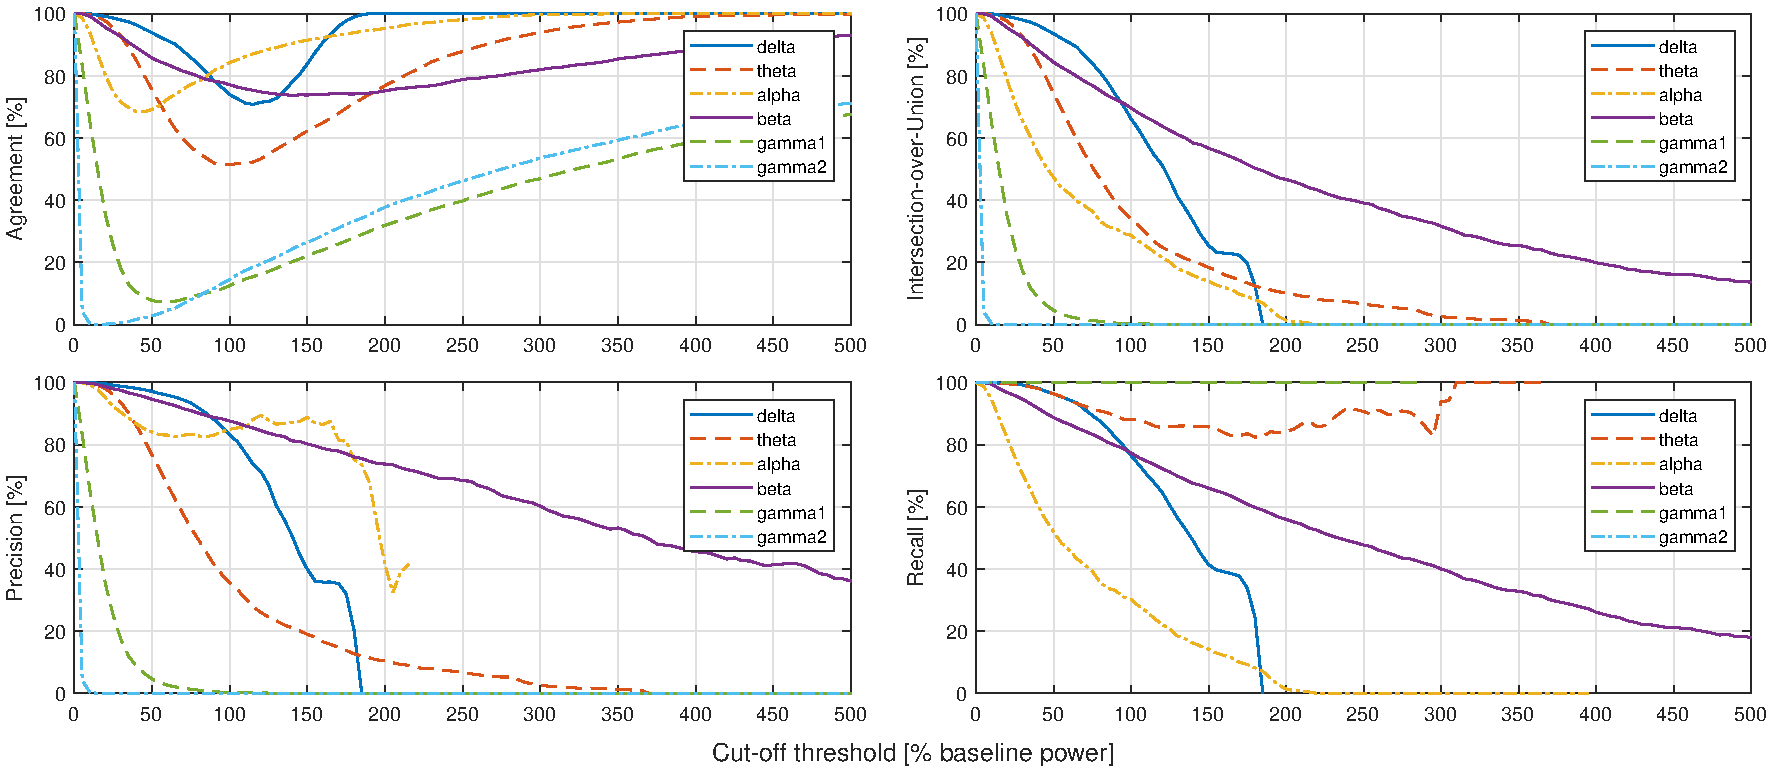
\includegraphics[width=16cm]{./img/MetricRelative}
\caption{Evaluation metrics for the automatic detection of bursts of high-amplitude activity using Virtual Deep Electrodes; the detection performed using real Deep Electrodes is considered the ground truth. 
A segment is labeled as `burst' if the total power exceeds a given threshold.
The detection was performed using different combinations of thresholds and band-pass filters (matching frequency bands).}
\label{fig:band}
\end{figure*}

In light of these observations, the recordings from Virtual Deep Electrodes and real Deep electrodes are first filtered to the frequency bands $\delta$ and $\beta$, and then the classification is performed using a threshold close to 150\% of baseline.

The results, displayed in figure \ref{fig:segment_stats}, indicate that the classifications are consistent within modalities in terms of the number of segments and their length.

\begin{figure*}[!t]
\centering
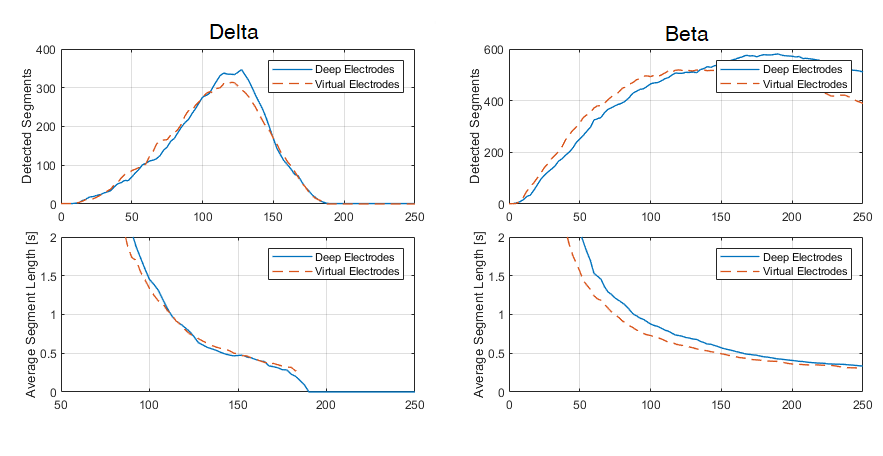
\includegraphics[width=16cm]{./img/improvised}
\caption{Evaluation metrics for the automatic detection of bursts of high-amplitude activity using Virtual Deep Electrodes; the detection performed using real Deep Electrodes is considered the ground truth. 
A segment is labeled as `burst' if the total power exceeds a given threshold.
The detection was performed using different combinations of thresholds and band-pass filters (matching frequency bands).}
\label{fig:segment_stats}
\end{figure*}

%============================================================================
%============================================================================

\section{Discussion}
\label{sec:discussion}

Virtual sensors such as the Virtual Deep electrodes described in this work have been described previously by many authors.
%
For example, in the context of epilepsy, the usability of virtual sensors constructed from EEG and MEG data has been explored \cite{sohrabpour2020noninvasive,tamilia2021noninvasive}.

In this work, we addressed a known issue from minimal-norm algorithms, which is the presence of multiple low-amplitude signals in the source space.
%
The proposed way to circumvent the issue is to integrate some threshold process into the pipeline.


The apparent success of this methodology may be attributed to the inherent low-noise nature of ECoG recordings, which include sensors placed directly at the brain cortex.

%============================================================================
%============================================================================

\section{Conclusion}

In this work, data from Electrical Source Reconstruction is used to simulate recordings from electrodes located inside the brain; this estimated data is referred to as recordings from Virtual Deep Electrodes.

Recordings from Virtual Deep Electrodes are more reliable on lower frequencies, up to approximately 30 Hz. Beyond that threshold, the computed quantities computed with virtual and real electrodes are still highly correlated but are less consistent.

Recordings from Virtual Deep Electrodes were then to perform an automatic detection of bursts of high-amplitude activity; under reasonable constraints, the results obtained are nearly identical to those obtained using real Deep Electrodes.

The great benefit of using Virtual Deep Electrodes is that they can be placed on any arbitrary location inside the brain, and they can be computed using less invasive modalities such as ECoG.


%============================================================================
%============================================================================

\section*{Acknowledgment}

We acknowledge the expert veterinary assistance of Dr. Misha Dunbar and Angela Guillory, and discussions with Dr. Vikram Jakkamsetti and Gauri Kathote.

JMP received the following NIH funding: RM1 NS133593 and R56 NS121993.
%NIH funding: RM1 NS133593 and R56 NS121993.

%============================================================================
%============================================================================

% references section

% can use a bibliography generated by BibTeX as a .bbl file
% BibTeX documentation can be easily obtained at:
% http://mirror.ctan.org/biblio/bibtex/contrib/doc/
% The IEEEtran BibTeX style support page is at:
% http://www.michaelshell.org/tex/ieeetran/bibtex/
\bibliographystyle{IEEEtran}

% argument is your BibTeX string definitions and bibliography database(s)
\bibliography{IEEEabrv, ./references.bib}
%
% <OR> manually copy in the resultant .bbl file
% set second argument of \begin to the number of references
% (used to reserve space for the reference number labels box)
%\begin{thebibliography}{1}

%\bibitem{IEEEhowto:kopka}
%H.~Kopka and P.~W. Daly, \emph{A Guide to \LaTeX}, 3rd~ed.\hskip 1em plus
%  0.5em minus 0.4em\relax Harlow, England: Addison-Wesley, 1999.

%\end{thebibliography}




% that's all folks
\end{document}


